\begin{itemize}
    \item \textbf{Wie lassen sich die beobachteten Reflexe leicht indizieren?}
    \item {In dem man die verschiedenen Reflexe den Gitterebenen (hkl) zuordnet erhält man mit dem
            Gitterebenenabstand $d_{hkl}=\frac{a}{\sqrt{h^2+k^2+l^2}}$ für kubische Gitter die Netzebenenabstände.
            Daraus folgt mit $n\lambda = 2d_{hkl}sin(\theta_{hkl})$ der Streuwinkel $\theta$, sodass bei 
            bekannter Wellenlänge jedem Winkel/Abstand paar ein millerscher Indize zugeordnet werden kann.}
    \item \textbf{Auslöschungsregeln für $Cu_3Au$}
    \item
    %\begin{align*}
                $$F = \sum_{j=1}^n f_j e^{i \vec{r_i} \vec{G}}$$ %\\
                $$r_0 = (0,0,0), r_1=a(1/2,1/2,0), r_2=a(1/2,0,1/2), r_3=a(0,1/2,1/2)$$% \\
                $$F = c(1+e^{\pi i a (h+k)}+e^{\pi i a (h+l)+e^{\pi i a (k+l)}})$$% \\
                $$\Rightarrow F \neq \text{0 für (h,k,l) alle gerade/ungerade} $$  
    %\end{align*}
    \item \textbf{Absorbtionseffekte sind abhängig von der Probengeometrie weil:}
    \item $$I = I_0 exp(-\mu d)$$
          $$\mu = n \sigma$$
          $\sigma$ = Wirkungsquerschnitt, n = Atome pro Kubikmeter, d = Probendicke
    \item \textbf{Wieso nur benachtbarte Reflexe vergleichen?}
    \item Da $A_T$ Winkelabhängig ist, kann man NUR für benachtbarte Reflexe annehmen das $A_T$
          identisch ist, und damit vernachlässigbar.
    \item \textbf{Widerstand von Kupfer}
    \item 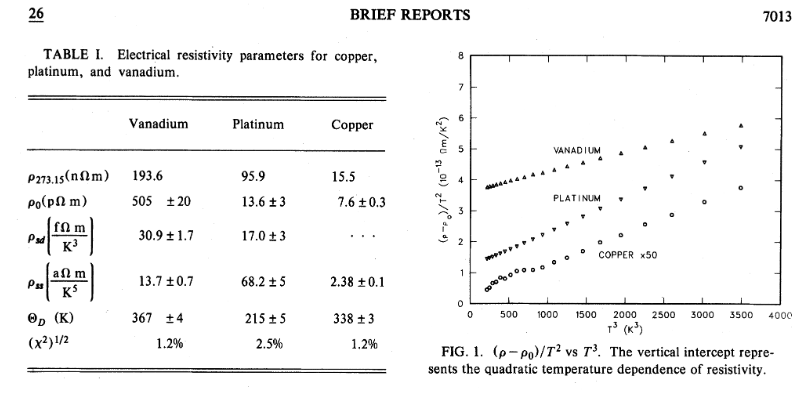
\includegraphics[width=0.8\textwidth]{images/copperkek.PNG}
    \item 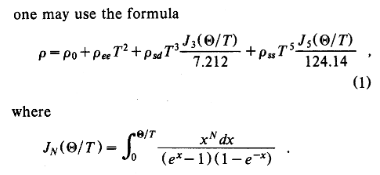
\includegraphics[width=0.8\textwidth]{images/copperwut.PNG}
    \item $$\rho(T) = 1 + \alpha(\frac{T}{\theta}) + cT^5$$
    \item \textbf{Effekt des Linienspektrum auf Messung}
    \item 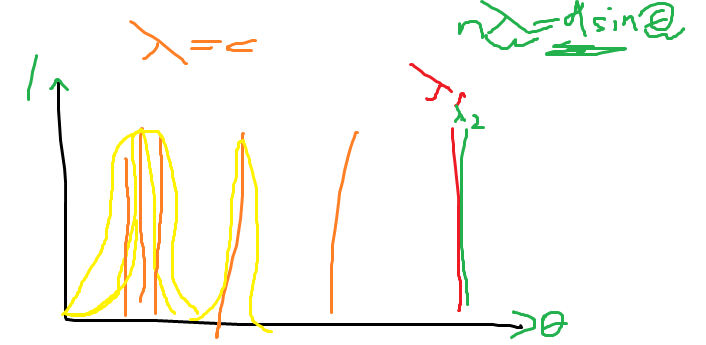
\includegraphics[width=0.8\textwidth]{images/linienspeckie.PNG}
    \item \textbf{Messung der 4 Punkt methode}
    \item 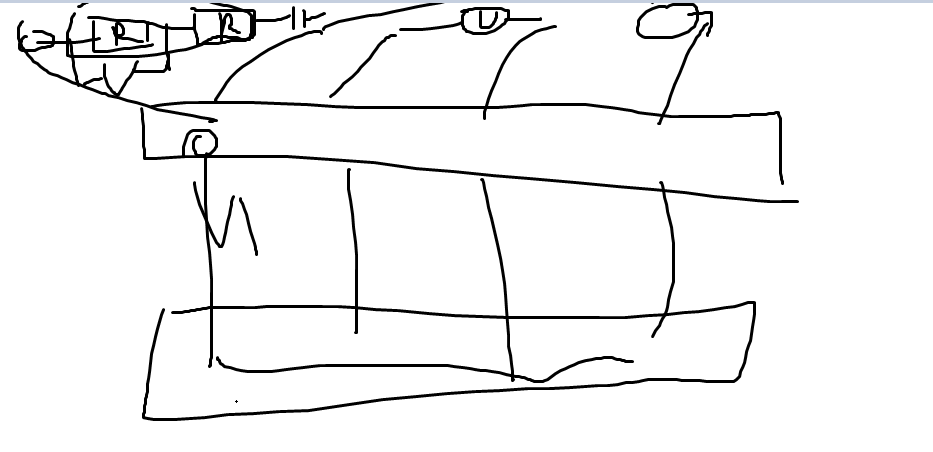
\includegraphics[width=0.8\textwidth]{images/4pointstyle.PNG}
    \item \textbf{Abhängigkeit vo nder geometrie}
    \item 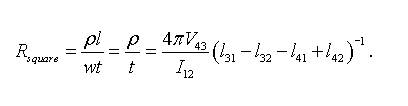
\includegraphics[width=0.8\textwidth]{images/geom.PNG}